\iffalse
\let\negmedspace\undefined
\let\negthickspace\undefined
\documentclass[journal,12pt,twocolumn]{IEEEtran}
\usepackage{float}
\usepackage{circuitikz}
\usepackage{cite}
\usepackage{amsmath,amssymb,amsfonts,amsthm}
\usepackage{algorithmic}
\usepackage{graphicx}
\usepackage{textcomp}
\usepackage{xcolor}
\usepackage{txfonts}
\usepackage{listings}
\usepackage{enumitem}
\usepackage{mathtools}
\usepackage{gensymb}
\usepackage{comment}
\usepackage[breaklinks=true]{hyperref}
\usepackage{tkz-euclide} 
\usepackage{listings}
\usepackage{gvv}                                        
\def\inputGnumericTable{}                                 
\usepackage[latin1]{inputenc}                                
\usepackage{color}                                            
\usepackage{array}                                            
\usepackage{longtable}                                       
\usepackage{calc}                                             
\usepackage{multirow}                                         
\usepackage{hhline}                                           
\usepackage{ifthen}                                           
\usepackage{lscape}
\newtheorem{theorem}{Theorem}[section]
\newtheorem{problem}{Problem}
\newtheorem{proposition}{Proposition}[section]
\newtheorem{lemma}{Lemma}[section]
\newtheorem{corollary}[theorem]{Corollary}
\newtheorem{example}{Example}[section]
\newtheorem{definition}[problem]{Definition}
\newcommand{\BEQA}{\begin{eqnarray}}
\newcommand{\EEQA}{\end{eqnarray}}
\newcommand{\define}{\stackrel{\triangle}{=}}
\theoremstyle{remark}
\newtheorem{rem}{Remark}
\begin{document}

\bibliographystyle{IEEEtran}
\vspace{3cm}
\title{NCERT 12.7 12Q}
\author{EE23BTECH11015 - DHANUSH V NAYAK$^{*}$% <-this % stops a space
}
\maketitle
\newpage
\bigskip
\renewcommand{\thefigure}{\arabic{figure}}
\renewcommand{\thetable}{\theenumi}
\bibliographystyle{IEEEtran}

\textbf{Question:} An LC circuit contains a $50 \mu H$ inductor and a $50 \mu F$ capacitor with an initial charge of $10 mC$. The resistance of the circuit is negligible. Let the instant the circuit is closed by $t = 0$.

\textbf{a)} What is the total energy stored initially? Is it conserved during LC oscillations?

\textbf{b)} What is the natural frequency of the circuit?

\textbf{c)} At what time is the energy stored \textbf{(i)} completely electrical (i.e., stored in the capacitor)? \textbf{(ii)} completely magnetic (i.e., stored in the inductor)?

\textbf{d)} At what times is the total energy shared equally between the inductor and the capacitor?

\textbf{e)} If a resistor is inserted in the circuit, how much energy is eventually dissipated as heat? \\
\hfill(NCERT 12.7 12Q)\\
\solution
\fi
\begin{table}[H]
\centering
\renewcommand\thetable{1}
\setlength{\extrarowheight}{9pt}
\resizebox{0.51\textwidth}{!}{
\begin{tabular}{|c|c|c|}
\hline
\textbf{Parameter} & \textbf{Description} & \textbf{Value} \\ \hline
$L$ &Inductance&$50 \mu H$  \\ \hline
$C$ &Capacitance&$50 \mu F$  \\ \hline
$E\brak{0}$ &Initial Energy of Capacitor&$?$  \\ \hline
$q\brak{0}$ &Initial Charge on Capacitor&$10 mC$  \\ \hline
$v\brak{0^-}$ &Initial Voltage on Capacitor&$200V$  \\ \hline
$\omega_{o}$ &Angular Resonant frequency&$?$  \\ \hline
\end{tabular}}
\caption{Parameter Table}
\label{tab:ncert-12.7.12}
\end{table}




\begin{enumerate}[label=\textbf{(\alph*)}]
    \item Initial energy stored :
    \begin{align}
        E\brak{0}&= \frac{1}{2}C\brak{v\brak{0^-}}^2\\
            &=  1 J 
    \end{align}
\begin{figure}[H]
    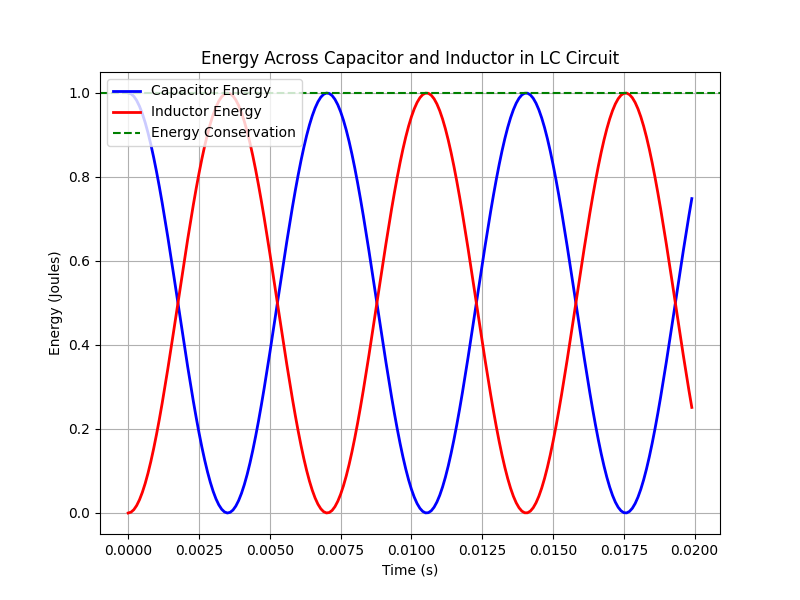
\includegraphics[width=1\columnwidth]{ncert-physics/12/7/12/figs/Plot_energy.png}
    \caption{Energy is Conserved During Oscillations total energy being limited to the initial energy}
    \label{fig:energy_plots}
\end{figure}
 \item 
The Laplace domain circuit :
\begin{figure}[H]
    \centering
    \resizebox{0.4\textwidth}{!}{\begin{circuitikz}[american]
    \draw (0,0)
    to[american inductor, l=$sL$, i=$i\brak{s}$] (2,0)
    to[capacitor, l=$\frac{1}{sC}$] (2,-2)
    -- (0,-2)
    to[V, v=$\frac{v(0^-)}{s}$] (0,0); 
\end{circuitikz}
}
    \caption{LC Circuit in lapalace domain}
    \label{fig:ncert_12.7.12_cktdiag_lap}
\end{figure}
Writing KVL in \figref{fig:ncert_12.7.12_cktdiag_lap}
\begin{align}
    \frac{-200}{s} - I\brak{s}Ls -I\brak{s}\frac{1}{sC} &= 0\\
    I\brak{s} &= \frac{-10^8}{25s^2 + 10^{10}}\label{eq:ncert12.7.12_i(s)}
\end{align}
Simplifying ,
\begin{align}
    I\brak{s} &= -200\brak{\frac{2\times10^4}{s^2+\brak{2\times10^4}^2}}
\end{align}
Now,
\begin{align}
    \sin\brak{at}u\brak{t} &\system{L} \frac{a}{s^2+a^2} \label{eq:gate_22_sint_result}\\
    \sin\brak{2\times10^4 t}u\brak{t} &\system{L} \frac{2\times10^4}{s^2+\brak{2\times10^4}^2}\label{eq:gate_22_q46.4}
\end{align}
Uisng \eqref{eq:gate_22_q46.4} on \eqref{eq:ncert12.7.12_i(s)}and taking inverse-Laplace transform:
\begin{align}
    i\brak{t} &= -200\sin(2\times10^4t)u\brak{t} 
\end{align}
From \figref{fig:ncert_12.7.12_cktdiag_lap} voltage across capacitor
\begin{align}
    V\brak{s} &= -\brak{I\brak{s}\frac{1}{sC} + \frac{V\brak{0^-}}{s}}\\
                &= \frac{5\times10^{3}s}{25s^2+10^{10}}\label{eq:gate_22_q46_V(s)}
\end{align}
Simplifying,
\begin{align}
    V\brak{s} &= 200 \brak{\frac{s}{s^2+\brak{2\times10^4}^2}}
\end{align}
\begin{align}
    \cos\brak{at}u\brak{t} &\system{L} \frac{s}{s^2+a^2} \label{eq:gate_22_cost_result}\\
    \cos\brak{2\times10^4t}u\brak{t} &\system{L} \frac{s}{s^2+\brak{2\times10^4}^2}\label{eq:gate_22_q46.5}
\end{align}
Using \eqref{eq:gate_22_q46.5} on \eqref{eq:gate_22_q46_V(s)}and taking inverse-Laplace transform:
\begin{align}
    v\brak{t} &=200\cos(2\times10^4t)u\brak{t}
\end{align}
The impedance of the circuit :
\begin{align}
    Z &=\frac{V\brak{s}}{I\brak{s}}= sL + \frac{1}{sC}
\end{align}
s can be expressed in angular frequency as :
\begin{align}
    s &= j\omega\\
    Z &= \brak{\omega L - \frac{1}{\omega C}}j\\
    \abs{Z} &= \omega L - \frac{1}{\omega C}
\end{align}
For resonant angular frequency imaginary part of impedance is zero :
\begin{align}
     \omega_{o}&=\frac{1}{\sqrt{LC}}\\
          &=20,000 \text{rad/sec}
\end{align}
\begin{figure}[H]
    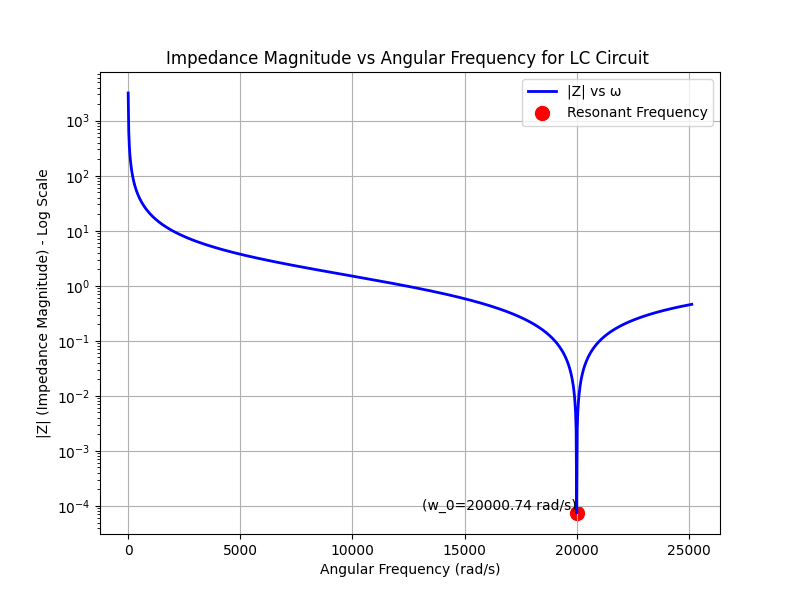
\includegraphics[width=0.8\columnwidth]{ncert-physics/12/7/12/figs/impedance_plot.png}
    \caption{The frequency at which impedance is minimum is resonant frequency which is at $20000$ rad/sec}
    \label{fig:Z vs omega}
\end{figure}
\item 
The energy stored is completely electrical when $i\brak{t}=0$.

The energy stored is completely magnetic when $v\brak{t}=0$

\begin{figure}[H]
    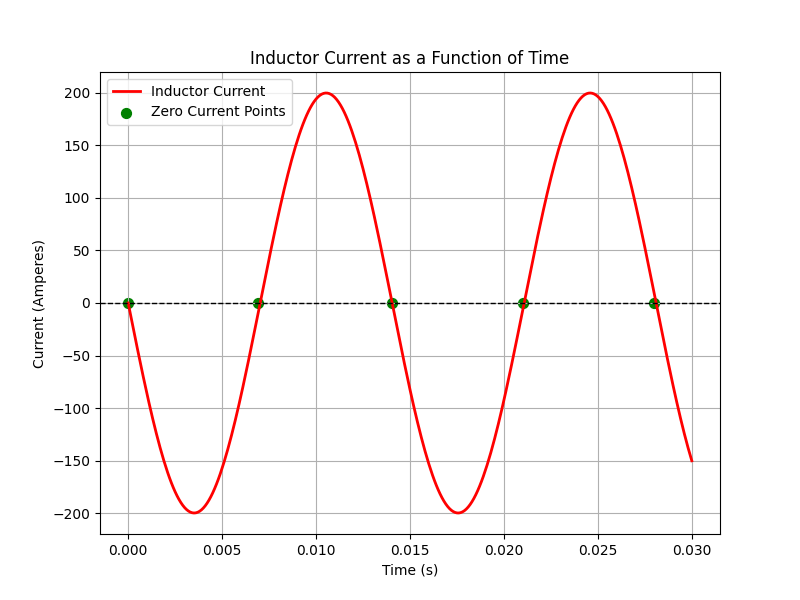
\includegraphics[width=1\columnwidth]{ncert-physics/12/7/12/figs/current_plot.png}
    \caption{Energy is completely electrical at the marked points. }
    \label{fig:current_plot}
\end{figure}
\begin{figure}[H]
    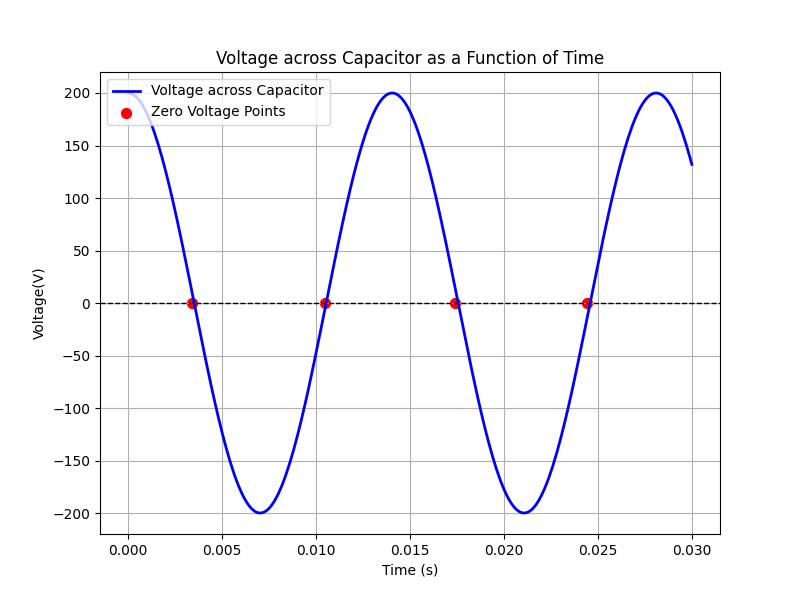
\includegraphics[width=1\columnwidth]{ncert-physics/12/7/12/figs/voltage_plot.png}
    \caption{Energy is completely magnetic at the marked points.}
    \label{fig:voltage_plot}
\end{figure}
\item When energy is equally shared then the capacitor has half of the maximum energy.
 \begin{align}
        \frac{1}{2}C\brak{v\brak{t}}^2 &= \frac{1}{2}\\
        \cos{\omega_{o} t}     &= \frac{1}{\sqrt{2}}\\
        t                 &= \frac{(2n+1)T}{8} , \text{$T$} = \frac{2\pi}{\omega_{o}}
\end{align}
Hence, the total energy is equally shared between the inductor and capacitor at the time,$t =\frac{T}{8},\frac{3T}{8},\frac{5T}{8} \ldots$ \\
\begin{figure}[H]
    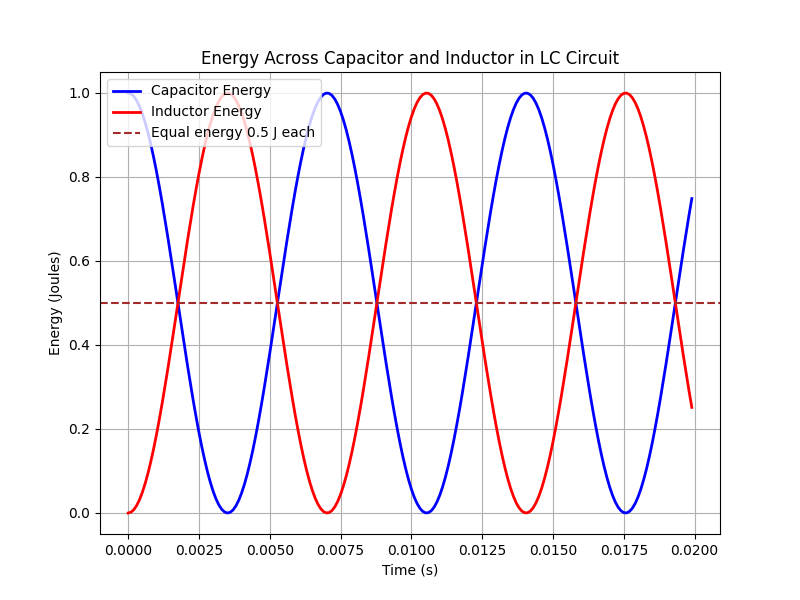
\includegraphics[width=1\columnwidth]{ncert-physics/12/7/12/figs/Plot_equal_energy.png}
    \caption{At the intersection points with 0.5 J horizontal line both capacitor and inductor have equal energy.}
    \label{fig:equal_energy_plot}
\end{figure}
\item Once the resistor is added to the LC circuit, it starts dissipating energy in the form of heat.
\begin{figure}[H] 
    \centering
\begin{circuitikz}[american, scale=1.5]
    \draw (0,0)
    to[inductor, l=$sL$, i=$I(s)$] (2,0)
    to[resistor, l=$R$] (2,-2)
    to[capacitor, l=$\frac{1}{sC}$] (1,-2)
    to[V, v=$\frac{v(0^-)}{s}$] (0,-2)
    -- (0,0);
\end{circuitikz}
    \caption{Laplace domain LCR Circuit with $R=1\Omega$}
    \label{fig:LCR_damping_ckt}
\end{figure}
\end{enumerate}
Applying KVL in  \figref{fig:LCR_damping_ckt}:
\begin{align}
    \brak{\frac{1}{sC}+sL+R}I\brak{s} &= \frac{v\brak{0^-}}{s}\\
    I\brak{s} &= \frac{10^{10}}{2500s^2+50\times10^6s+10^{12}}\\
              &= -\frac{400}{\sqrt{3}}\brak{\frac{\sqrt{3}\times10^4}{\brak{s+10^4}^2+\brak{\sqrt{3}\times10^4}^2}}
\end{align}
By frequency-shifting property:
\begin{align}
    e^{-\alpha t}x\brak{t} &\system{L} X\brak{s+\alpha} \label{eq:laplace_freq_shifting_prop}
\end{align}
Applying \eqref{eq:laplace_freq_shifting_prop} on \eqref{eq:gate_22_q46.4}
\begin{align}
    e^{-10^4t}\sin(10^4\sqrt{3}t)u\brak{t} &\system{L} \brak{\frac{\sqrt{3}\times10^4}{\brak{s+10^4}^2+\brak{\sqrt{3}\times10^4}^2}} \label{eq:gate_ee_q46.7}
\end{align}
Using \eqref{eq:gate_ee_q46.7} and  Taking inverse Laplace transform:
\begin{align}
    i\brak{t} &= -\frac{400}{\sqrt{3}}e^{-10^4 t}\sin(10^4\sqrt{3}t)
    \end{align}


\begin{figure}[H]
    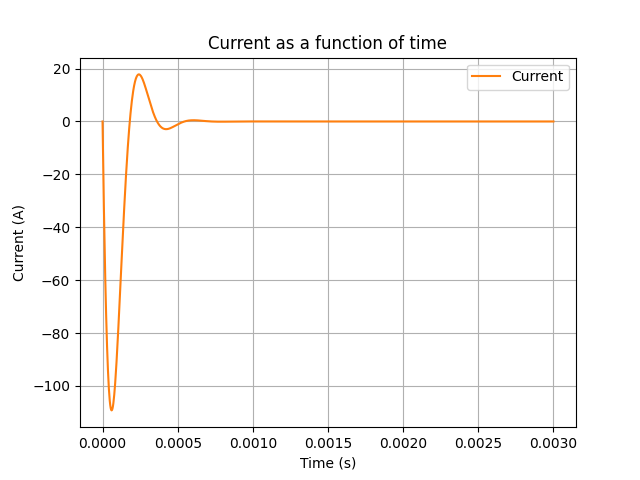
\includegraphics[width=1\columnwidth]{ncert-physics/12/7/12/figs/Current_in_circuit_during_damping.png }
    \caption{Graph of current in the circuit. Becomes zero after all the energy is dissipated, $R=1\Omega$}
    \label{fig:current_in_damping}
\end{figure}

\begin{figure}[H]
    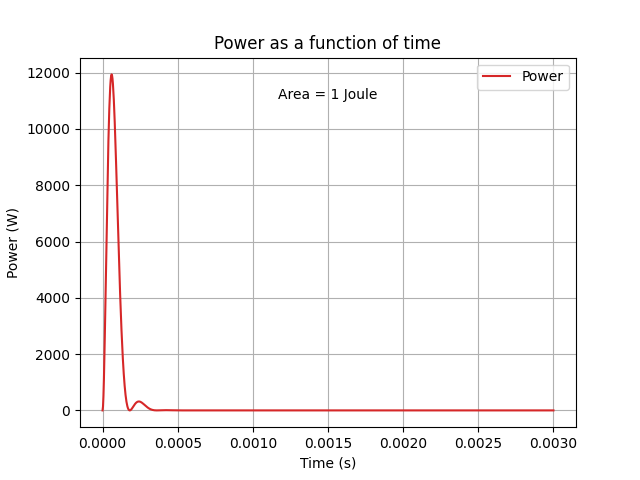
\includegraphics[width=1\columnwidth]{ncert-physics/12/7/12/figs/Power_Dissipated_across_Resistor.png }
    \caption{Power Dissipated across resistor, $R=1\Omega$. The area under the curve is 1J.}
    \label{fig:power_in_damping}
\end{figure}

%\end{document}

